\pagebreak
\section{Peso dell'esplorazione variabile} \label{sec:peso_esplorazione}
Il termine $\rho$, presente nell'Equazione \ref{eq:objective_function}, è un coefficiente che  indica l'importanza del processo di esplorazione all'interno dell'obiettivo globale.
Poiché la copertura degli utenti è l'obiettivo primario, inizialmente si è deciso di dare all'esplorazione una rilevanza minore, in modo che vengano favorite quelle azioni maggiormente orientate alla copertura; è stato dunque impostato un \textbf{peso constante} \texttt{EXPLORATION\_WEIGHT} (Snippet \ref{snip:expl_weight}), strettamente minore di 1.

\lstinputlisting[
language=Python 
, label={snip:expl_weight}
, caption = {varianti di peso dell'obiettivo di esplorazione}
, float = h
, frame=tb
, belowcaptionskip=3mm
]{code/expl_weight.py}

Successivamente è stato osservato come, nelle fasi iniziali, solitamente il valore di RCR fosse basso, risultando quindi sfavorevole incentivare la copertura di pochi utenti, rispetto alla ricerca di nuovi.
Per evitare tale comportamento, è stato implementato un \textbf{coefficiente di esplorazione decrescente} al crescere del numero di utenti coperti (Snippet \ref{snip:expl_weight}), ma indipendente dal loro totale, che permette di dare una rilevanza maggiore all'obiettivo di esplorazione nelle fasi iniziali, e ridurne il peso all'aumentare degli utenti coperti, applicando nuovamente un approccio più conservativo.
Inizialmente, come si vede in Figura \ref{fig:expl_weight_comparison}, quando la configurazione dei sensori ha un livello di RCR basso, l'importanza della funzione di esplorazione sarà relativamente elevata, per poi decrescere rapidamente; così facendo si ottiene un approccio flessibile alla configurazione attuale del sistema.

\begin{figure}
    \centering
    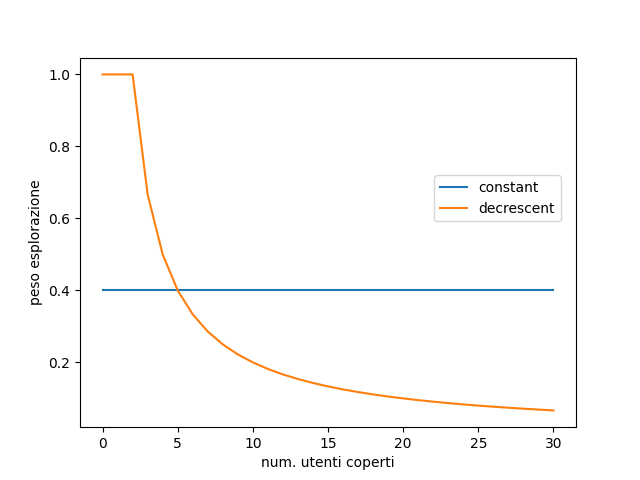
\includegraphics[width=0.8\textwidth]{img/ch3/expl_weight_comparison.png}
    \caption{Confronto tra i due tipi di peso al variare del numero di utenti coperti}
    \label{fig:expl_weight_comparison}
\end{figure}